\documentclass[11pt,a4paper]{article}
\usepackage{amsmath}
\usepackage{enumerate}
\usepackage{graphicx}

\usepackage{geometry} 
\geometry{a4paper,scale=0.8}

\usepackage{pythonhighlight}


\title{Module 2}

\date{}

\begin{document}

\maketitle

The main idea of detecting fraudulent credit card transactions is to find abnormal points. For anomalies, there exists some attributes 
which are significantly different from normal points and this makes them easier to be isolated in random partitions. 

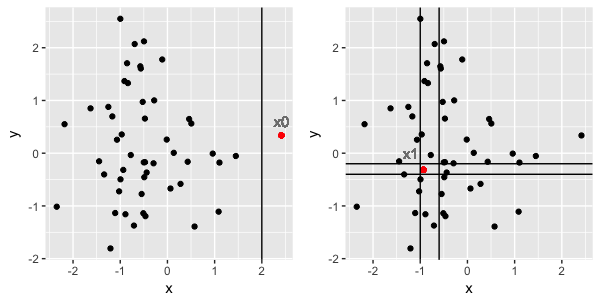
\includegraphics[width=\linewidth]{../figure/Rplot1.png}

From the plot above, we can see that anomalies $x_0$ requires only one partitions to be isolated while $x_1$ needs 4.

Due to this characteristic, I choose Isolation Tree to detect anomalies.\\

\noindent\textbf{Isolation Tree:} Denote $T$ as a node of an isolation tree. $T$ is either a leaf with no child or consists of an attribute $q$ 
and a split value $p$, and use test $q<p$ to split data $X$ into $\{X_l, X_r\}$.\\

For example, given a set of data $X = \{x_1,\dots,x_n\}$ with $d$ attributes. Each time an attribute $q$ is randomly drawn and sample 
$p\sim Unif(\min(q),\max(q))$. Then the test $q<p$ is used to split data $X$ into $\{X_l, X_r\}$. And for $X_l$ and $X_r$, repeat the 
previous steps until either: (a) $|X| = 1$ or (b) the tree reaches its height limit.

Then, I define a function:

\begin{equation}\label{c}
    c(n) =  2H(n-1) - 2(n-1)/n
\end{equation}

\noindent , where $H$ is the harmonic number.\\

\noindent\textbf{Path Length:} Path Length $h(x)$ for a instance $x$ is the summation of (a) the number of edges $x$ travels to reach one leaf $T$ and 
(b) $c(n)$ where $c(.)$ is defined in \eqref{c} and $n$ is the number of instance in dataset $X$ reaching that leaf $T$.\\

\noindent\textbf{Anomaly Score:} Anomaly Score for a instance $x$ is $s(x, N) = 2^{-\frac{h(x)}{c(N)}}$, where $N$ is the number of instance used to 
build the tree.\\

Anomalies tend to be isolated with short path length and $s(x, N)\Rightarrow 0$, when $h(x)\Rightarrow 0$. So instance with Anomaly 
Score closed to 0 is defined as anomalies, which is fraudulent credit card transactions in this case.
 
Since data comes in stream, previous data can be taken as train data to build Isolated Tree and use this tree to calculate the Anomaly 
Score of new data. Then, new data will be added to the previous data to generate a new tree for future predictions.

\begin{python}
    def iTree(X, e, l): # X: input data, e: current tree height, l: height limit
        node = Node()
        if(|X|<=1 or e>l):
            node.size = len(X.index)
        else:
            splitAtt = X.columns[random.randint(0, (len(X.columns)-1))]
            minimum = min(X[splitAtt])
            maximum = max(X[splitAtt])
            splitValue = np.random.uniform(low=minimum, high=maximum)
            Xl = X.loc[X[splitAtt]<=splitValue, :]
            Xr = X.loc[X[splitAtt]>splitValue, :]
            ee = e + 1
            Child_left = iTree(X=Xl, e=ee+1, l=l)
            node.setChildren(Child_left)
            Child_right = iTree(X=Xr, e=ee+1, l=l)
            node.setChildren(Child_right)
        return(node)

    def PathLength(x, T, e): # x: test data, T: isolated tree, e: current path length
        node = Node()
        if(T.isleaf()):
            return(e + c(T.size))
        else:
            q = T.splitAtt
            p = T.splitValue
            if(x[q]<=p):
                return(PathLength(x, T.Child_left, e+1))
            else:
                return(PathLength(x, T.Child_right, e+1))
\end{python}






\end{document}